\section{終わりに\label{sec:conclusion}}
本修論ではSYK模型の2点関数および4点関数の詳細な議論や, 量子カオス的性質を述べた. 
第\ref{sec:twopointfunc}節では2点関数や自己エネルギーの従うシュウィンガー・ダイソン方程式や
SYK模型の作用を示した. 
この作用から得られる2点関数や自己エネルギーのラージ$N$における
リーディングダイアグラムはメロンダイアグラムと呼ばれるものであった. 
またSYK模型は低エネルギー極限においてリパラメトリゼーション不変性を持ち, 特にシュウィンガー・ダイソン方程式
の解として共形対称性を持つものを選ぶ事ができ, リパラメトリゼーション不変性は自発的に破れた. 
低エネルギーでは共形古典解を用いる事で具体的な解析を行う事ができたが, 
解析は他にもラージ$q$においても行う事ができた(本修論では扱わなかったが, $q=2$としても解析解が存在する). 

第\ref{sec:fourpointfunc}節では4点関数のラージ$N$のリーディングオーダーでの振る舞いを調べた. 
司るダイアグラムはラダーダイアグラムであり, 4点関数のリーディングオーダーはこのダイアグラムの
総和で記述されるものであった. 
このラダーダイアグラムの総和の計算には低エネルギー極限での共形対称性が活用されたが, 
この級数は低エネルギー極限では計算上の技術的な問題から発生する見かけ上の発散項を持ち, 
この問題を回避するには低エネルギーから少し高エネルギー側に移る必要があった. 
従ってリパラメトリゼーション不変性は自発的に, また陽にも破れる事となった. 
この際に現れるソフトモードはシュワルツ理論に従う事を第\ref{sec:effective_theory}節では論じた. 

第\ref{sec:thermodynamics}節ではSYK模型に登場するエントロピーや比熱といった熱力学的な量を計算した. 
これは続く量子カオスでの議論に重量な量として登場するスペクトラル形状因子の振る舞いについて重要な
役割を担った. 

第\ref{sec:syk_as_quantum_chaos}節以降では量子カオスと関連した議論を展開した. 
まず始めにスペクトラル形状因子という量を導入し, これについて量子カオスの基礎となる数学と期待されている
ランダム行列理論での説明を行った. 
スペクトラル形状因子にはslope, rampおよびplateauと呼ばれる3つの領域が存在し, 
SYK模型のスペクトラル形状因子の持つ3つの領域もランダム行列理論で(近似的に)記述する事ができた. 
続いてスペクトラル形状因子のフェルミオンの2点関数および自己エネルギーを用いた記述が行われ, 
plateau以外の領域は対応した解となる配位を見つける事ができた. 

第\ref{sec:gravity}節ではSYK模型の重力双対であるJackiw--Teitelboimディラトン重力理論の
量子カオス的な振る舞いを調べた. 
具体的にはスペクトラル形状因子に相当する量のslopeとrampにあたる領域が, SYK模型での解と
対応している事を見た. 
ただしここでもplateauは論じなかった. 

以下では今後の課題を述べる. 
まず, plateauの振る舞いがどのような$G$と$\Sigma$の配位で与えらえるかはやはり調べるべきものである. 
また重力側で言えばどのような時空の幾何がplateauを与えるかでもある. 
plateauの存在は純粋に量子論的な効果であり, 古典的な重力では記述できない可能性もある. 

次はスペクトラル形状因子において, 特にdisorder averageを取らなかった場合の議論である. 
つまり次のような量を計算したとする:
\begin{align}
	Z(\beta + iT)Z(\beta - iT).
\end{align}
これを数値的にプロットすると図\ref{fig:non_disorder_averaged_g}のようにrampとplateauは
大きく揺らぐ事になる. 
\begin{figure}[ht]
	\centering
	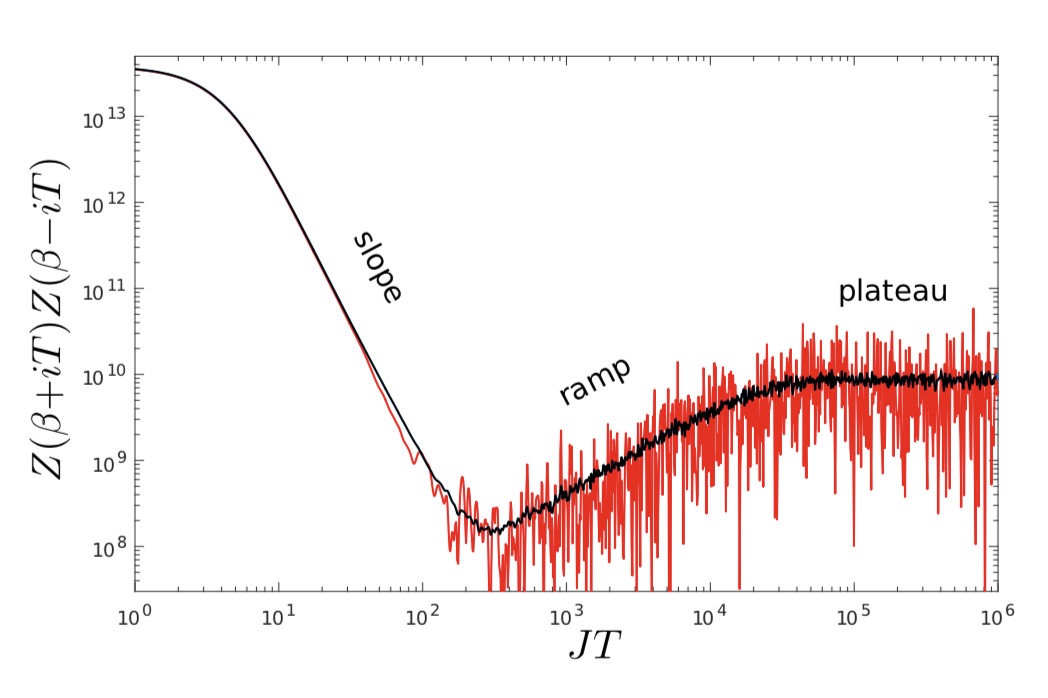
\includegraphics[width=10cm]{figures/non_disorder_averaged_g}
	\caption{disorder averageを取らなかった場合のスペクトラル形状因子を赤で示した. 
	黒はdisorder averageを取ったものである. 
	rampやplateauあたりはとても揺らいでいる. この図は\cite{stanford_chaos}より引用した. }
	\label{fig:non_disorder_averaged_g}
\end{figure}

重要な点は, 重力側の計算においても, このようなdisorder averageを取らないスペクトラル形状因子
を計算していたのにも関わらず, rampやplateauに大きな揺らぎを与えるものが見つからなかった事である. 
これは, もしかしたら重力理論というものは少なくとも何らかの期待値計算を施された理論である事を示唆しているの
かもしれない\cite{stanford_chaos}. 

SYK模型はAdS/CFT対応の研究として現時点では最も調べやすい模型であり, ブラックホールの量子論的
振る舞いの理解へ期待されるものである. 
しかしながら, plateauに代表されるような$t \gg 1$での振る舞いはまだまだ謎が多い. 
しかし, slopleやrampにはある種のAdS/CFT対応が見られるため、今後は量子重力やブラックホールといった
ものは量子カオスの分野に組み込まれる可能性もある.
ただし, 量子カオス自体に厳密な定義が存在しないため, こちらはこちらで詳細を調べていかないといけない.
SYK模型はそこにも一筋の光を差し込むと期待される.

またSYK模型は様々な変形版が存在し, 例えば高次元のSYK模型や, フェルミオンに電荷を持たせたようなものも
調べられている\cite{gaikwad}\cite{berkooz}. 
SYK模型そのものの研究もこれからの課題である. 

\pagebreak
